The research strategy defines how the research goal is to be achieved \cite{SaundersMark2023}.
This aspect of the research design is crucial as it outlines the steps to be taken to address the research questions effectively.
Several research strategies have been defined including: Experiment, Survey, Case study, Action research, Grounded theory, Ethnography and Archival research.
Each of these strategies is designed with a specific purpose in mind and is best suited to achieving the intended research objective.

Since the primary goal of this thesis is to design and develop an artefact, the research strategy used is the \gls{dsr} \cite{Hevner2010}.
\gls{dsr} is a research methodology that focuses on what is called ``relevance'', which is the creation and evaluation of an artifact to solve complex real-world problems.
Moreover, the research should enhance the existing body of knowledge, a principle referred to as ``rigor''.
This duality emerges from the fundamental idea that \gls{dsr} combines two distinct research paradigms: behavioral science and design science, each serving unique objectives to achieve the overall research goals.
A proposed Information Systems Research framework (Fig.~\ref{fig:information-system-research-framework}) illustrates this dual nature, emphasizing the necessity of addressing both a practical business need and the application of relevant knowledge in the research process.

\begin{figure}[htbp]
    \centering
 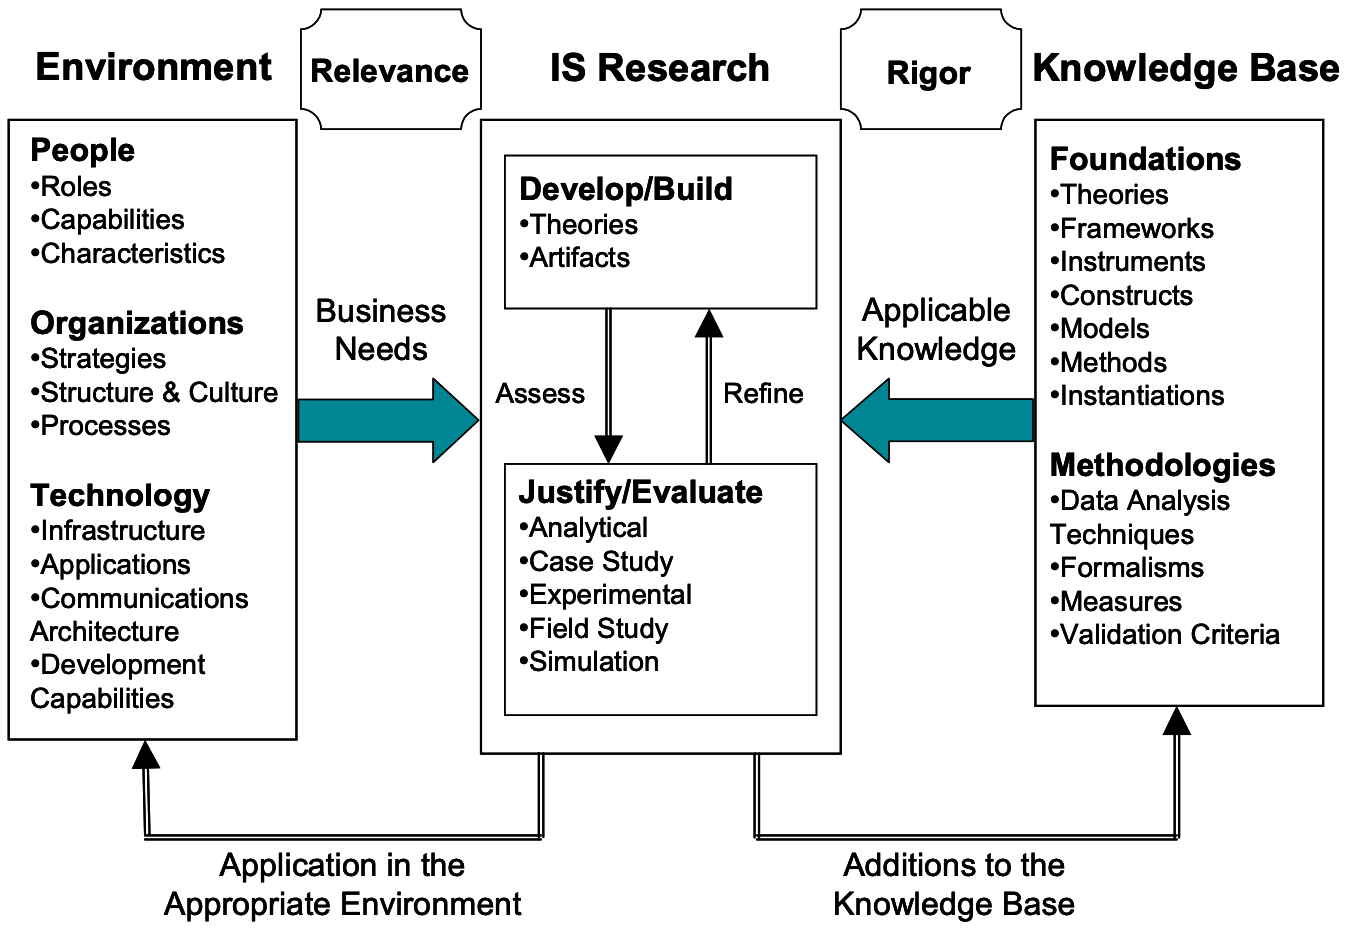
\includegraphics[width=.9\textwidth]{03_Figures/research-methods/information-system-research-framework.png}
     \rule{35em}{0.5pt}
    \caption{Information Systems Research Framework (\textcite{Hevner2010})} 
 \label{fig:information-system-research-framework}
\end{figure}

As already mentioned, the \gls{dsr} focuses on the creation and evaluation of an artifact to solve complex real-world problems.
The \gls{dsr} process is iterative, involving multiple cycles of development and evaluation, as illustrated in Fig.~\ref{fig:design-science-research-cycles}.

\begin{figure}[htbp]
    \centering
 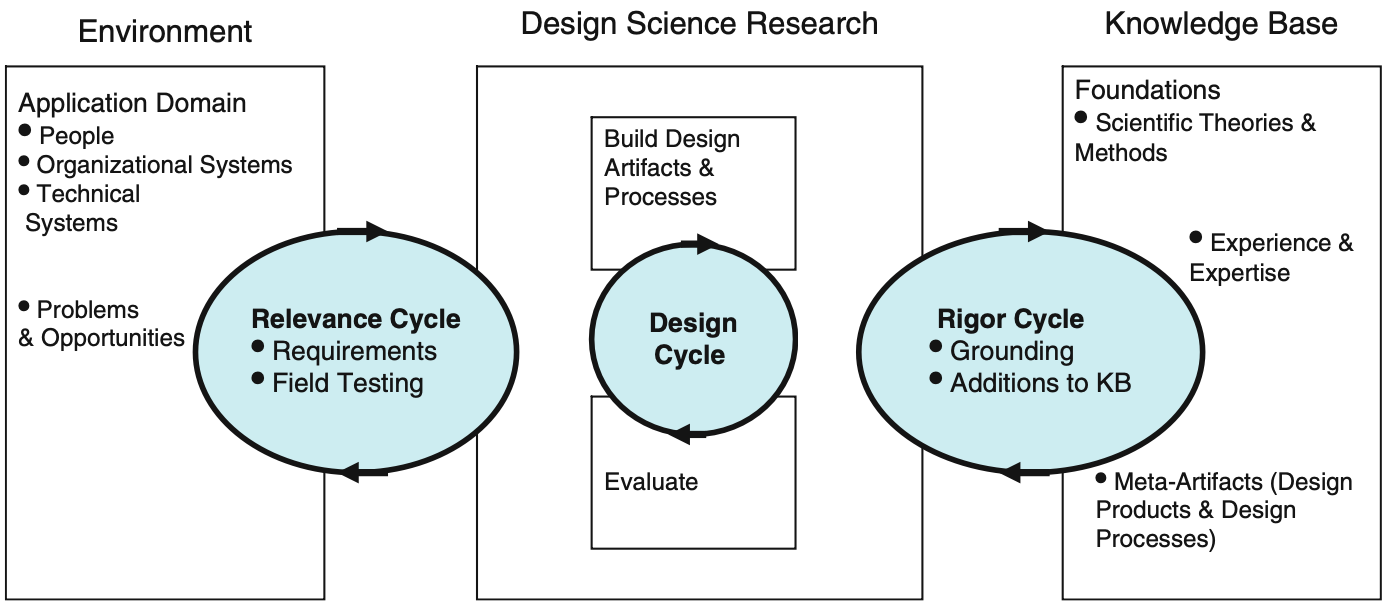
\includegraphics[width=.9\textwidth]{03_Figures/research-methods/design-science-research-cycles.png}
     \rule{35em}{0.5pt}
    \caption{\acrlong{dsr} Cycles (\textcite{Hevner2010}) } 
 \label{fig:design-science-research-cycles}
\end{figure}

On the right side, the Rigor Cycle focuses on existing knowledge, incorporating theories, methodologies, and expert experiences.
In the context of this thesis, it represents the literature review.
On the left side, the Relevance Cycle highlights the application domain, encompassing the people, organizations, systems, and the challenges or opportunities they face.
At the center, there is the Design Cycle, which addresses research through the development and evaluation of the artifact.
These three components are interconnected, forming a continuous \gls{dsr} cycle that ensures the integration of knowledge, practical relevance, and iterative refinement.

According to \textcite{Hevner2010}, the \gls{dsr} is defined in five process steps: awareness of problem, suggestion, development, evaluation, and conclusion.
\textcite{Hevner2010} modified a framework originally proposed by \textcite{Vaishnavi2007}, illustrating the five process steps along with the expected outputs and knowledge flows, as illustrated in Fig.~\ref{fig:design-science-research-framework}.

\begin{figure}[htbp]
    \centering
 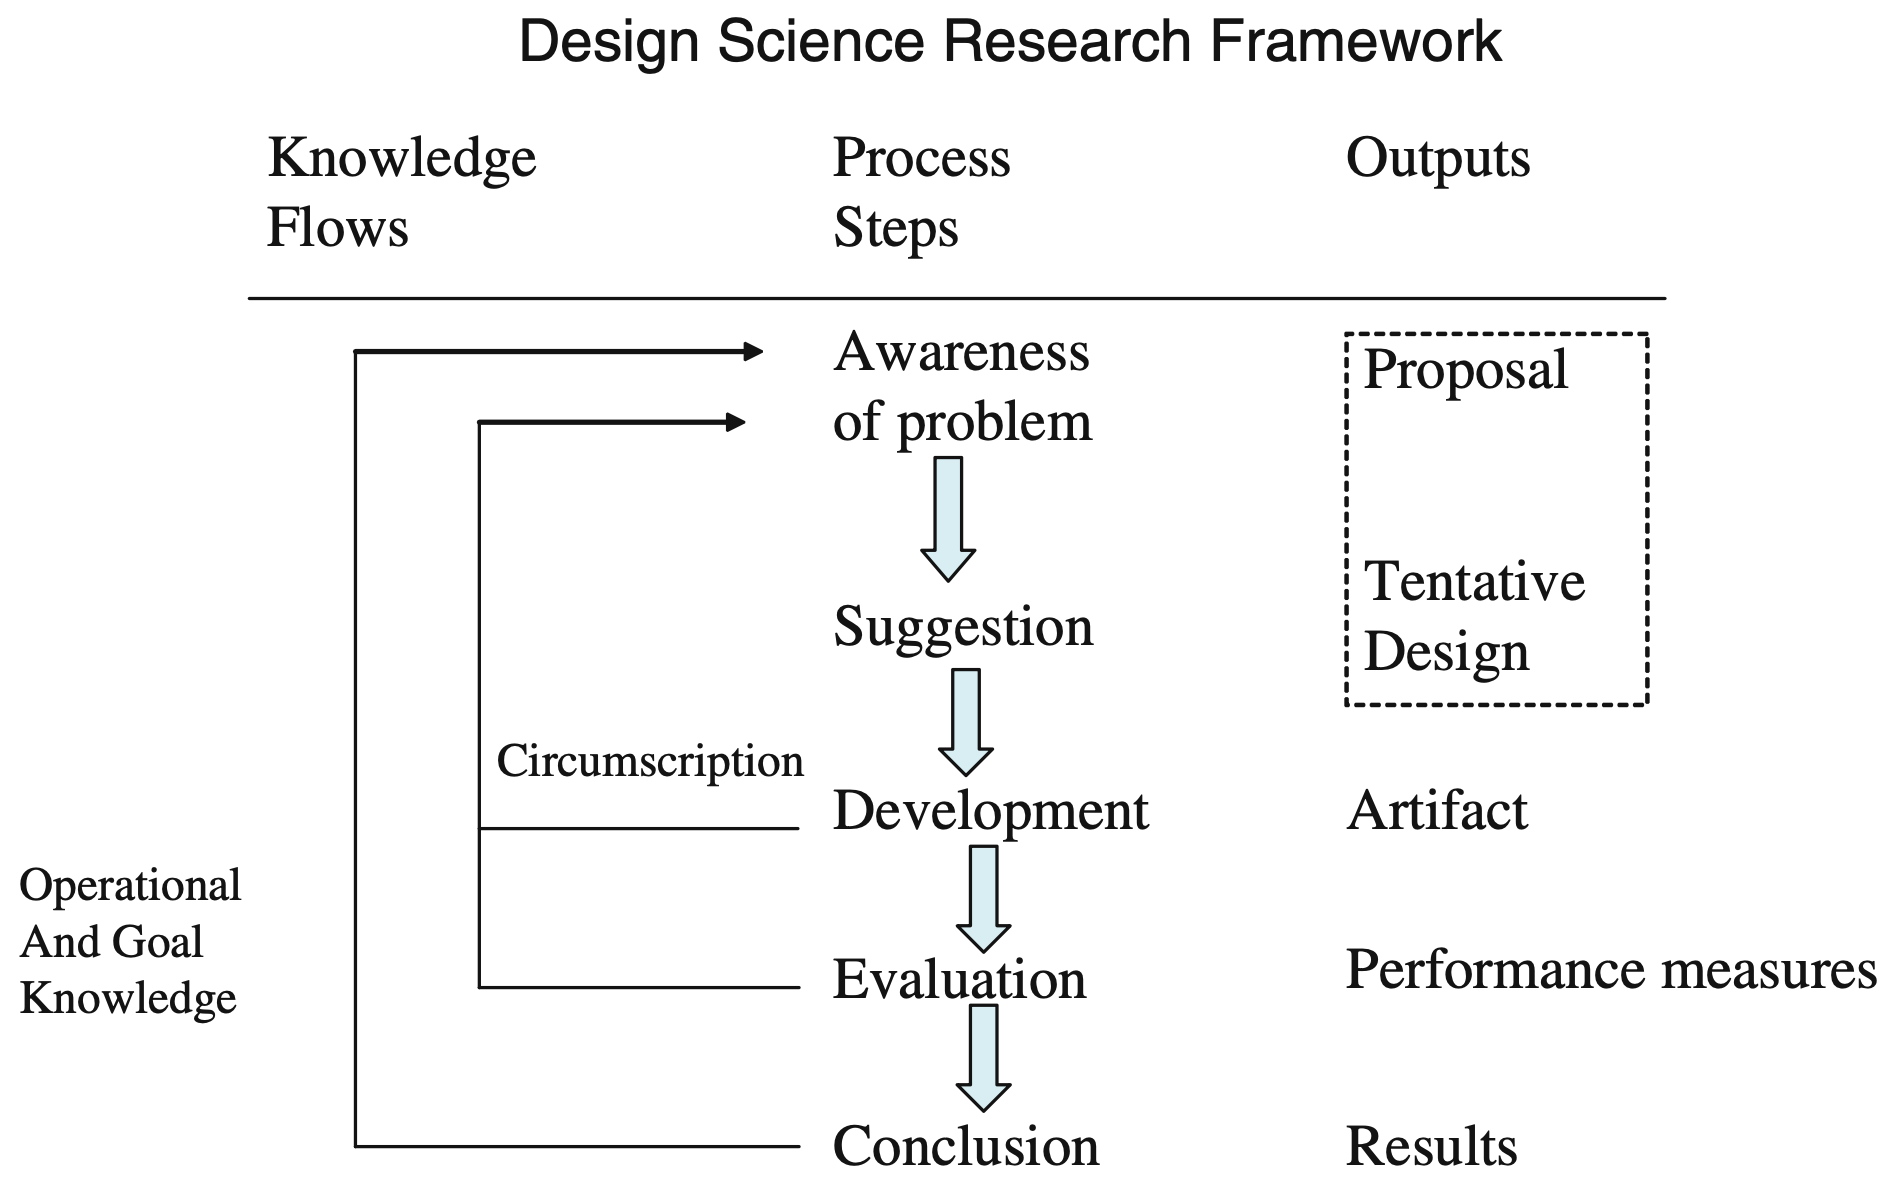
\includegraphics[width=.9\textwidth]{03_Figures/research-methods/design-science-research-framework.png}
     \rule{35em}{0.5pt}
    \caption{\acrlong{dsr} Framework (\textcite{Hevner2010}) adapted from (\textcite{Vaishnavi2007})} 
 \label{fig:design-science-research-framework}
\end{figure}

The research of this thesis will follow the \gls{dsr} methodology, in accordance with the five steps of the framework proposed by \textcite{Hevner2010}.
Each of the \gls{dsr} steps are described in the Chapter \ref{chap:research-methods}.


Fig.~\ref{fig:design-science-research-framework-adapted-by-author} illustrates the \gls{dsr} framework adapted by the author, which will be used to guide the research process in this thesis.
\begin{figure}[htbp]
    \centering
 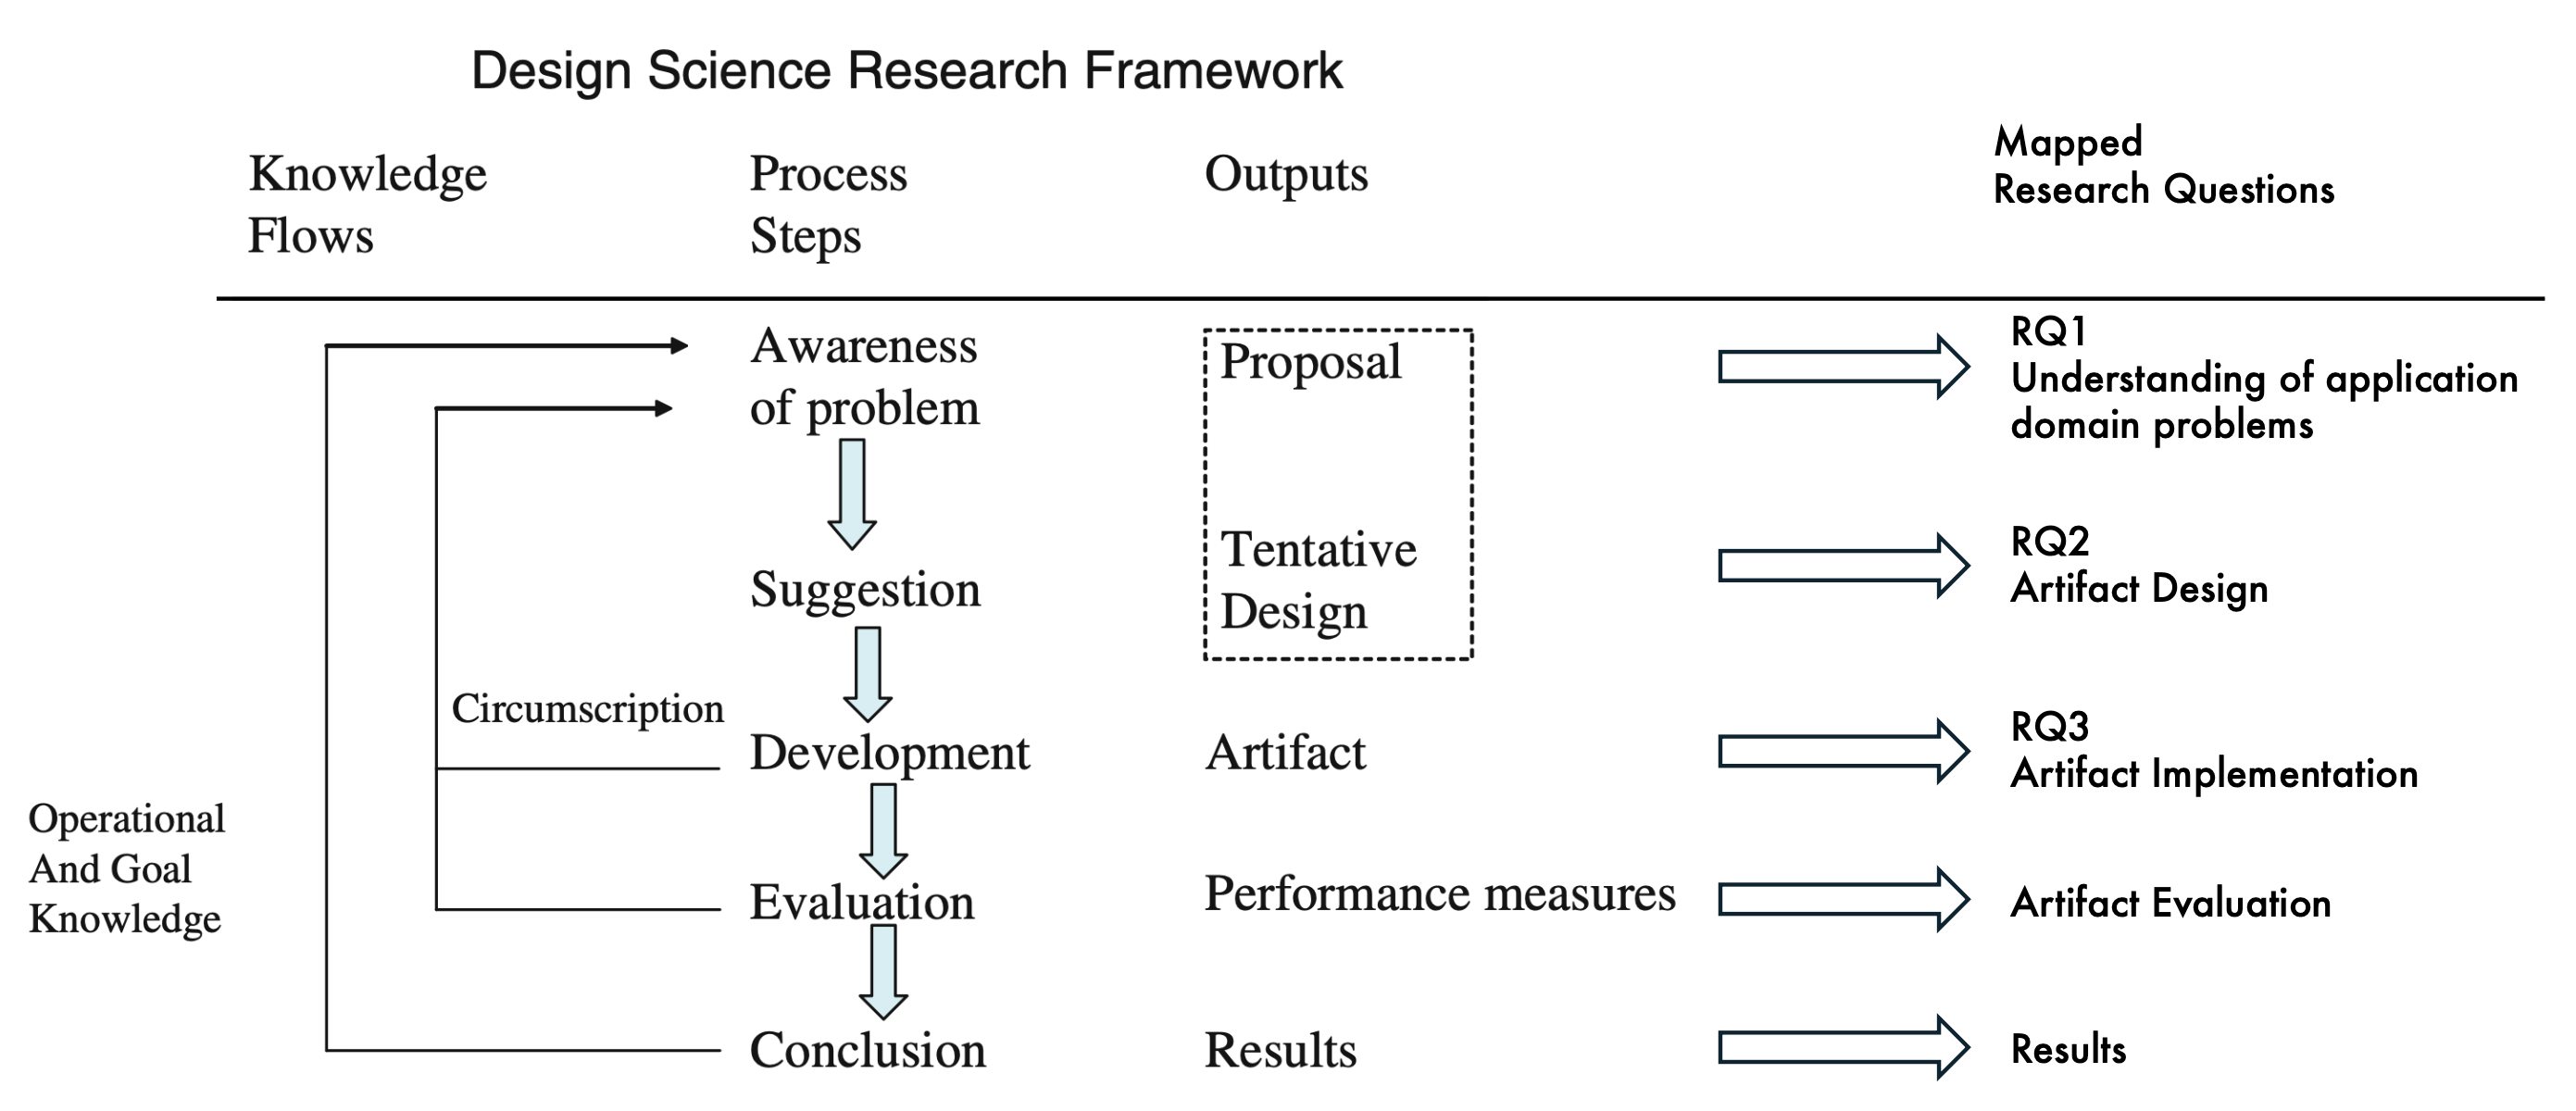
\includegraphics[width=.9\textwidth]{03_Figures/research-methods/design-science-research-framework-by-author.png}
     \rule{35em}{0.5pt}
    \caption{\acrlong{dsr} Framework adapted by the author} 
 \label{fig:design-science-research-framework-adapted-by-author}
\end{figure}

